\documentclass[12pt]{article}
\usepackage{amsmath}
\usepackage{amssymb}
\usepackage{tikz}
\usepackage{stmaryrd}
\usepackage{url}
\usepackage{color}
\usepackage{subfigure}
\usepackage{graphicx}
\usepackage{epstopdf}
\usepackage{fancyhdr}
\usepackage{enumerate}
%\usepackage{algorithmic}
\usepackage{algorithm}
\usepackage{algpseudocode}
\usepackage{pifont}
\usepackage{float}
\usepackage[colorlinks=true,urlcolor=blue]{hyperref}
\usepackage{comment}

\oddsidemargin  0in \evensidemargin 0in \topmargin -0.5in
\headheight 0.25in \headsep 0.25in
\textwidth   6.5in \textheight 9in %\marginparsep 0pt \marginparwidth 0pt
\parskip 1.5ex  \parindent 0ex \footskip 20pt

\newcommand{\note}[1]{\textsf{{\textcolor{red}{[[#1]]}}}}
\newcommand{\boxcomment}[1]{\noindent\fbox{\parbox{\textwidth}{#1}}\medskip\\}

\newcommand{\xhdr}[1]{\paragraph{\bf{#1}}}
\newcommand{\subquestion}[1]{\subsubsection*{{#1}}}
% \newcommand{\Solution}[1]{}
\newcommand{\Solution}[1]{\paragraph{\bf $\bigstar $ SOLUTION:} {\sf #1} \bigskip}
\newcommand{\Mistake}[2]{\paragraph{\bf $\blacksquare$ COMMON MISTAKE #1:} {\sf #2} \bigskip}
% Math shortcuts
\newcommand{\transpose}[1]{{#1}^{\mathrm{T}}}

%%---------------------------------------------------------------------------
%%      Theorems and other environments:
%%---------------------------------------------------------------------------
\newtheorem{thm}{Theorem}%[lecture]
\newtheorem{prop}{Proposition}%[lecture]
\newtheorem{lemma}{Lemma}%[lecture]
\newtheorem{result}{Result}%[lecture]
\newtheorem{cor}{Corollary}%[lecture]
\newtheorem{claim}{Claim}%[lecture]
\newenvironment{proof}{{\bf Proof:}}{\hfill\rule{2mm}{2mm}}
\newenvironment{solution}{{\bf Solution:}}{\hfill\rule{2mm}{2mm}}
\newcounter{example}
\newenvironment{example}[1][]
 {\refstepcounter{example}{\bf Example~\arabic{example}~#1}}{}
 \renewcommand{\theexample}{\arabic{example}}
\newcounter{problem}
\newenvironment{problem}[1][]
 {\refstepcounter{problem}{\bf Problem~\arabic{lecture}.\arabic{problem}~#1}}{}
 \renewcommand{\theproblem}{\arabic{lecture}.\arabic{problem}}

\newcounter{definition}
\newenvironment{definition}[1][Definition]{\begin{trivlist}
\item[\hskip \labelsep {\bfseries #1}]}{\end{trivlist}}
%\newcounter{algorithm}
%\newenvironment{algorithm}[1][]
% {\refstepcounter{algorithm}{\bf Algorithm~\arabic{algorithm}~#1}}{}
% \renewcommand{\thedefinition}{\arabic{algorithm}}

%%%-----------------------------------------------------------------------------
%%% Header
\newfont{\bssten}{cmssbx10}
\newfont{\bssnine}{cmssbx10 scaled 900}
\newfont{\bssdoz}{cmssbx10 scaled 1200}
\pagestyle{fancy}  % use this?
 \fancyhead{\bssnine CS 246: Mining Massive Data Sets - Problem Set 2}
 \fancyhead[RE]{} \fancyhead[LO]{}
 \fancyhead[LE]{\bssnine \arabic{page}} \fancyhead[RO]{\bssnine \arabic{page}}
 \lfoot{} \cfoot{} \rfoot{}
%%%-----------------------------------------------------------------------------
%
\begin{document}
\thispagestyle{empty}
\boxcomment{
{\bf \textsf{CS246: Mining Massive Data Sets \hfill Winter 2020}}\medskip \\

\centerline{\LARGE \bf \textsf{Problem Set 2}}\medskip

{\hfill Please read the homework submission policies at \url{http://cs246.stanford.edu}.\hfill}
}

%%-----------------------------------------------------------------------------
%% Questions
\includecomment{solutions}
%\excludecomment{solutions}
\section{Singular Value Decomposition and Principal Component Analysis (20 points)}

In this problem we will explore the relationship between two of the most popular dimensionality-reduction techniques, SVD and PCA, at a basic conceptual level. Before we proceed with the question itself, let us briefly recap the SVD and PCA techniques and a few important observations:
\begin{itemize}
\item First, recall that the eigenvalue decomposition of a \emph{real}, \emph{symmetric}, and \emph{square matrix} $B$ (of size $d \times d$) can be written as the following product:
\[
	B = Q \Lambda \transpose{Q}
\]
where $\Lambda = \text{diag}(\lambda_1, \dots, \lambda_d)$ contains the eigenvalues of $B$ (which are always real) along its main diagonal and $Q$ is an orthogonal matrix containing the eigenvectors of $B$ as its columns. 

\item Principal Component Analysis (PCA): Given a data matrix $M$ (of size $p \times q$), PCA involves the computation of the eigenvectors of $M M^T$ or $M^T M$. The matrix of these eigenvectors can be thought of as a rigid rotation in a high dimensional space. When you apply this transformation to the original data,
the axis corresponding to the principal eigenvector is the one along which the
points are most “spread out.” More precisely, this axis is the one along which
the variance of the data is maximized. Put another way, the points can best be
viewed as lying along this axis, with small deviations from this axis. Likewise,
the axis corresponding to the second eigenvector (the eigenvector corresponding
to the second-largest eigenvalue) is the axis along which the variance of
distances from the first axis is greatest, and so on.
\item Singular Value Decomposition (SVD): SVD involves the decomposition of a data matrix $M$ (of size $p \times q$) into a product: $U \Sigma V^T$ where $U$ (of size $p \times k$) and $V$ (of size $q \times k$) are column-orthonormal matrices\footnote{A matrix $U \in \mathbb{R}^{p \times q}$ is column-orthonormal if and only if $U^TU = I$ where $I$ denotes the identity matrix} and $\Sigma$ (of size $k \times k$) is a diagonal matrix. The entries along the diagonal of $\Sigma$ are referred to as singular values of $M$. The key to understanding what SVD offers is in viewing the r columns of $U$, $\Sigma$, and $V$ as representing concepts that are hidden in the original matrix M.
\end{itemize}

For answering the questions below, let us define a real matrix $M$ (of size $p \times q$) and let us assume this matrix corresponds to a dataset with $p$ data points and $q$ dimensions. 

\subquestion{(a) [3 points]} 
Are the matrices $M M^T$ and $M^T M$ symmetric, square and real? Explain.

\subquestion{(b) [5 points]}
Prove that the nonzero eigenvalues of $M M^T$ are the same as the nonzero eigenvalues of $M^T M$. You may ignore multiplicity of eigenvalues. Are their eigenvectors the same? 

\subquestion{(c) [2 points]}
Given that we now understand certain properties of $M^T M$, write an expression for $M^T M$ in terms of $Q$, $Q^T$ and $\Lambda$ where $\Lambda = \text{diag}(\lambda_1, \dots, \lambda_d)$ contains the eigenvalues of $M^T M$ along its main diagonal and $Q$ is an orthogonal matrix containing the eigenvectors of $M^T M$ as its columns?\\
\textit{Hint: Check the definition of eigenvalue decomposition provided in the beginning of the question to see if it is applicable.}


\subquestion{(d) [5 points]}
SVD decomposes the matrix $M$ into the product $U \Sigma V^T$ where $U$ and $V$ are column-orthonormal and $\Sigma$ is a diagonal matrix. Given that $M = U \Sigma V^T$, write a simplified expression for $M^T M$ in terms of $V$, $V^T$ and $\Sigma$.

\subquestion{(e) [5 points]}
In this question, let us experimentally test if SVD decomposition of $M$ actually provides us the eigenvectors (PCA dimensions) of $M^T M$. We strongly recommend students to use Python and suggested functions for this exercise.\footnote{Other implementations of SVD and PCA might give slightly different results. Besides, you will just need fewer than five python commands to answer this entire question} Initialize matrix $M$ as follows: 
\[ M =
\begin{bmatrix}
1 & 2\\
2 & 1\\
3 & 4\\
4 & 3\\
\end{bmatrix}
\] 
\begin{itemize}
\item Compute the SVD of $M$ (\emph{Use scipy.linalg.svd function in Python and set the argument \texttt{full\_matrices} to False}). The function returns values corresponding to $U$, $\Sigma$ and $V^T$. What are the values returned for $U$, $\Sigma$ and $V^T$?
\emph{Note: Make sure that the first element of the returned array $\Sigma$ has a greater value than the second element.}
\item Compute the eigenvalue decomposition of $M^T M$ (\emph{Use scipy.linalg.eigh function in Python}). The function returns two parameters: a list of eigenvalues (let us call this list $Evals$) and a matrix whose columns correspond to the eigenvectors of the respective eigenvalues (let us call this matrix $Evecs$). Sort the list $Evals$ in descending order such that the largest eigenvalue appears first in the list. Also, re-arrange the columns in $Evecs$ such that the eigenvector corresponding to the largest eigenvalue appears in the first column of $Evecs$. 
What are the values of $Evals$ and $Evecs$ (after the sorting and re-arranging process)?\\
%\emph{Note: Check the ordering of the eigenvalues in the list when you associate eigenvectors with the eigenvalues.}


\item Based on the experiment and your derivations in part (c) and (d), do you see any correspondence between $V$ produced by SVD and the matrix of eigenvectors $Evecs$ (after the sorting and re-arranging process) produced by eigenvalue decomposition? If so, what is it?\\
\emph{Note: The function scipy.linalg.svd returns $V^T$ (not $V$).}


\item Based on the experiment and the expressions obtained in part (c) and part (d) for $M^T M$, what is the relationship (if any) between the eigenvalues of $M^T M$ and the singular values of $M$? Explain. \\
\textit{Note: The entries along the diagonal of $\Sigma$ (part (e)) are referred to as singular values of $M$. The eigenvalues of $M^T M$ are captured by the diagonal elements in $\Lambda$ (part (d))}

\end{itemize}

{\bf What to submit:} 
\begin{enumerate}[(i)]
\item Written solutions to questions 1(a) to 1(e) with explanations wherever required
\item Upload the code via Gradescope [1(e)]
\end{enumerate}

\section{$k$-means on Spark (20 points)}

\textbf{Note:} This problem should be implemented in Spark. You should \textbf{not} use the Spark MLlib clustering library for this problem. You may store the centroids in memory if you choose to do so.

\begin{center}
	{\footnotesize \ding{92} \hspace{1em} \ding{92} \hspace{1em} \ding{92}}
\end{center}


This problem will help you understand the nitty gritty details of implementing
clustering algorithms on Spark. In addition, this problem will also help you
understand the impact of using various distance metrics and initialization
strategies in practice. Let us say we have a set $\mathcal{X}$ of $n$ data
points in the $d$-dimensional space $\mathbb{R}^d$. Given the number of
clusters $k$ and the set of $k$ centroids $\mathcal{C}$, we now proceed to
define various distance metrics and the corresponding cost functions that they
minimize. 

\textbf{Euclidean distance}
Given two points $A$ and $B$ in $d$ dimensional space such that $A = [a_1, a_2 \cdots a_d]$ and $B = [b_1, b_2 \cdots b_d]$, the Euclidean distance between $A$ and $B$ is defined as:
\begin{equation}\label{eqn:ed}
||a - b|| = \sqrt{\sum_{i=1}^{d} (a_i - b_i) ^2}
\end{equation}

The corresponding cost function $\phi$ that is minimized when we assign points to clusters using the Euclidean distance metric is given by:
\begin{equation}\label{eqn:ced}
\phi = \sum_{x\in \mathcal{X}} \min_{c\in\mathcal{C}} ||x-c||^2
\end{equation}
Note, that in the cost function the distance value is squared. This is intentional, as it is the squared Euclidean distance the algorithm is guaranteed to minimize.

\textbf{Manhattan distance}
Given two random points $A$ and $B$ in $d$ dimensional space such that $A = [a_1, a_2 \cdots a_d]$ and $B = [b_1, b_2 \cdots b_d]$, the Manhattan distance between $A$ and $B$ is defined as:
\begin{equation}\label{eqn:md}
|a - b| = \sum_{i=1}^{d} |a_i - b_i|
\end{equation}

The corresponding cost function $\psi$ that is minimized when we assign points to clusters using the Manhattan distance metric is given by:
\begin{equation}\label{eqn:cmd}
\psi = \sum_{x\in \mathcal{X}} \min_{c\in\mathcal{C}} |x - c|
\end{equation}

\textbf{Iterative $k$-Means Algorithm:} 
We learned the basic $k$-Means algorithm in class which is as follows: $k$ centroids are initialized, each point is assigned to the nearest centroid and the centroids are recomputed based on the assignments of points to clusters. In practice, the above steps are run for several iterations.  We present the resulting iterative version of $k$-Means in Algorithm \ref{kmeans}.
\begin{algorithm}
\small
\caption{Iterative $k$-Means Algorithm}
\label{kmeans}
\begin{algorithmic}[1]
\Procedure{Iterative $k$-Means}{}
\State Select $k$ points as initial centroids of the $k$ clusters. 
\For{iterations $:=$ 1 to \texttt{MAX\_ITER}}
\For{each point $p$ in the dataset}
\State Assign point $p$ to the cluster with the closest centroid
\EndFor
\State Calculate the cost for this iteration.
\For{each cluster $c$}
\State Recompute the centroid of $c$ as the mean of all the data points assigned to $c$
\EndFor
\EndFor
\EndProcedure
\end{algorithmic}
\end{algorithm}

\textbf{Iterative $k$-Means clustering on Spark:} Implement iterative $k$-means
using Spark. Please use the dataset from \texttt{q2/data} within the bundle for this problem.

The folder has 3 files:
\begin{enumerate}
\item \texttt{data.txt} contains the dataset which has 4601 rows and 58
columns.
Each row is a document represented as a 58 dimensional vector of features. Each
component in the vector represents the importance of a word in the document. The ID to download \texttt{data.txt} into a Colab is 1E-voIV2ctU4Brw022Na8RHVVRGOoNkO1
\item \texttt{c1.txt} contains $k$ initial cluster centroids. These centroids were
chosen by selecting $k = 10$ random points from the input data. The ID to download \texttt{c1.txt} into a Colab is 1yXNlZWMqUcAwDScBrkFChOHJwR1FZXmI
\item \texttt{c2.txt} contains initial cluster centroids which are as far apart
as possible, using Euclidean distance as the distance metric. (You can do this by choosing 1\textsuperscript{st} centroid c1 randomly, and then finding the point c2 that is farthest from c1, then selecting c3 which is farthest from c1 and c2, and so on). The ID to download \texttt{c2.txt} into a Colab is 1vfovle9DgaeK0LnbQTH0j7kRaJjsvLtb
\end{enumerate}

Set number of iterations (\texttt{MAX\_ITER}) to $20$ and number of clusters
$k$ to $10$ for all the experiments carried out in this question. Your driver
program should ensure that the correct amount of iterations are run.

\subquestion{(a) Exploring initialization strategies with Euclidean distance [10 pts]} 

\begin{enumerate}
\item \textbf{[5 pts] } 
Using the Euclidean distance (refer to Equation \ref{eqn:ed}) as the distance measure, compute the cost function $\phi(i)$ (refer to Equation \ref{eqn:ced}) for every iteration $i$. This means that, for your first iteration, you'll be computing the cost function using the initial centroids located in one of the two text files. Run the $k$-means on \texttt{data.txt} using \texttt{c1.txt} and \texttt{c2.txt}. Generate a graph where you plot the cost function $\phi(i)$ as a function of the number of iterations $i$=1..20 for \texttt{c1.txt} and also for \texttt{c2.txt}. You may use a single plot or two different plots, whichever you think best answers the theoretical questions we’re asking you about.

\textit{(Hint: Note that you do not need to write a separate Spark job to compute $\phi(i)$. You should be able to calculate costs while partitioning points into clusters.)}

\item \textbf{[5 pts] } What is the percentage change in cost after 10 iterations of the K-Means algorithm when the cluster centroids are initialized using \texttt{c1.txt} vs. \texttt{c2.txt} and the distance metric being used is Euclidean distance? Is random initialization of
$k$-means using \texttt{c1.txt} better than initialization using \texttt{c2.txt}
in terms of cost $\phi(i)$? Explain your reasoning.

\textit{(Hint: to be clear, the percentage refers to (cost[0]-cost[10])/cost[0].)}

\end{enumerate}

\subquestion{(b) Exploring initialization strategies with Manhattan distance [10 pts]} 
\begin{enumerate}
\item \textbf{[5 pts] } 
Using the Manhattan distance metric (refer to Equation \ref{eqn:md}) as the distance measure, compute the cost function $\psi(i)$ (refer to Equation \ref{eqn:cmd}) for every iteration $i$. This means that, for your first iteration, you'll be computing the cost function using the initial centroids located in one of the two text files. Run the $k$-means on \texttt{data.txt} using \texttt{c1.txt} and \texttt{c2.txt}. Generate a graph where you plot the cost function $\psi(i)$ as a function of the number of iterations $i$=1..20 for \texttt{c1.txt} and also for \texttt{c2.txt}. You may use a single plot or two different plots, whichever you think best answers the theoretical questions we’re asking you about.

\textit{(Hint: This problem can be solved in a similar manner to that of part (a). Also note that It's possible that for Manhattan distance, the cost do not always decrease. K-means only ensures monotonic decrease of cost for squared Euclidean distance. Look up K-medians to learn more.)}

\item \textbf{[5 pts] } What is the percentage change in cost after 10 iterations of the K-Means algorithm when the cluster centroids are initialized using \texttt{c1.txt} vs. \texttt{c2.txt} and the distance metric being used is Manhattan distance? Is random initialization of
$k$-means using \texttt{c1.txt} better than initialization using \texttt{c2.txt}
in terms of cost $\psi(i)$? Explain your reasoning.

\end{enumerate}

\textbf{What to submit:}\\
\begin{enumerate}[(i)]
\item Upload the code for 2(a) and 2(b) to Gradescope
\item A plot of cost vs. iteration for two initialization strategies [2(a)]
\item Percentage improvement values and your explanation [2(a)]
\item A plot of cost vs. iteration for two initialization strategies [2(b)]
\item Percentage improvement values and your explanation [2(b)]
\end{enumerate}


\section{Latent Features for Recommendations (35 points) }

\textbf{Note}: Please use native Python (Spark not required) to solve this problem. It usually takes several minutes to run, however, time may differ depending on the system you use.

\begin{center}
	{\footnotesize \ding{92} \hspace{1em} \ding{92} \hspace{1em} \ding{92}}
\end{center}
The goal of this problem is to implement the \textit{Stochastic Gradient Descent} algorithm to
build a Latent Factor Recommendation system. We can use it to
recommend movies to users. We encourage you to  read the slides of the lecture
``Recommender Systems 2'' again before attempting the problem.

Suppose we are given a matrix $R$ of ratings. The element $R_{iu}$
of this matrix corresponds to the rating given by user $u$ to item $i$. The size of $R$ is $m\times n$, where $m$ is the number of movies, and $n$ the number of users.

Most of the elements of the matrix are unknown because each user can only rate a few movies. 

Our goal is to find two matrices $P$ and $Q$, such that $R \simeq QP^T$. The dimensions of $Q$ are $m \times k$, and the dimensions of $P$ are $n \times k$. $k$ is a parameter of the algorithm.

We define the error as
\begin{equation}
	E = \bigg(\sum_{(i,u) \in \textnormal{ratings}} (R_{iu} - q_i\cdot p_u^{T})^2\bigg) + \lambda
\left[\sum_u\|p_u\|_{2}^{2} + \sum_i\|q_i\|_{2}^{2}\right].
\label{eq:rec}
\end{equation}
The $\sum_{(i,u) \in \textnormal{ratings}}$ means that we sum only on the pairs
$(\textnormal{user},\textnormal{item})$ for which the user has rated the item, \emph{i.e.} the $(i,u)$ entry of the matrix $R$ is known.  $q_i$ denotes the $i$\textsuperscript{th} row of the matrix $Q$ (corresponding to an item), and $p_u$ the $u$\textsuperscript{th} row of the matrix $P$ (corresponding to a user $u$). $q_i$ and $p_u$ are both row vectors of size $k$. $\lambda$ is the regularization parameter. $\|\cdot\|_{2}$ is the $L_2$ norm and
$\|p_u\|_{2}^{2}$ is square of the $L_2$ norm, \emph{i.e.,} it is the sum of squares of elements of $p_u$.


\subquestion{(a) [10 points]}

Let $\varepsilon_{iu}$ denote the derivative of the error $E$ with respect to $R_{iu}$. What is the expression for $\varepsilon_{iu}$? What are the update equations for $q_i$ and $p_u$ in the Stochastic Gradient Descent algorithm? Please show your derivation and use $\varepsilon_{iu}$ in your final expression of $q_i$ and $p_u$.

\subquestion{(b) [25 points]}

Implement the algorithm. Read each entry of the matrix
$R$ from disk and update $\varepsilon_{iu}$, $q_i$ and $p_u$ for each entry.

%\textbf{
To emphasize, you are not allowed to store the matrix $R$ in memory. You have to read each element $R_{iu}$ one at a time from disk and apply your update equations (to each element) each iteration. Each iteration of the algorithm will read the whole file.
%}

Choose $k=20$, $\lambda = 0.1$ and number of iterations = 40. Find a good value for the learning rate $\eta$, starting with $\eta = 0.1$. (You may not modify $k$ or $\lambda$) The error $E$ on the training set ratings.train.txt discussed below should be less than $65000$ after 40 iterations; you should observe both $q_i$ and $p_u$ stop changing. 

Based on values of $\eta$, you may encounter the following cases:
\begin{itemize}
\item If $\eta$ is too big, the error function can converge to a high value or
may not monotonically decrease. It can even diverge and make the components of vectors $p$ and $q$ equal to $\infty$.
\item If $\eta$ is too small, the error function doesn't have time to significantly decrease and reach convergence. So, it can monotonically decrease but not converge \emph{i.e.} it could have a high value after 40 iterations because it has not converged yet.
\end{itemize}

Use the dataset at \texttt{q3/data} within the bundle for this problem. It contains the following files:
\begin{itemize}
\item \texttt{ratings.train.txt}: This is the matrix $R$. Each entry is made of a user id, a movie id, and a rating. \end{itemize}

\textbf{Plot the value of the objective function $E$ (defined in equation~\ref{eq:rec}) on the training set as a function of the number of iterations. What value of $\eta$ did you find?}

You can use any programming language to implement this part, but Java, C/C++, and Python are recommended for speed. (In particular, Matlab can be rather slow reading from disk.)
It should be possible to get a solution that takes on the order of minutes to run with these languages.


\textit{Hint: These hints will help you if you are not sure about how to proceed for
certain steps of the algorithm, although you don't have to follow them if you have another method.
\begin{itemize}
%	\item Determine the dimensions of $P$ and $Q$. You can compute the maximal userID and movieID from a pass through the data. (You should not assume these constants are known at the start of your program.) This allows you to store $P$ and $Q$ in "sparse" matrices; for items $i$ and users $u$ not present in the training set, the rows $q_i$ and $p_u$ will never be updated.
	\item Initialization of $P$ and $Q$: We would like $q_i$ and $p_u$ for all users $u$ and
items $i$ such that $q_i \cdot p_u^{T} \in [0,5]$. A good way to achieve that is to initialize
all elements of $P$ and $Q$ to random values in $[0, \sqrt{5/k}]$.
	\item	Update the equations: In each update, we update $q_i$ using $p_u$ and $p_u$ using $q_i$. Compute the new values for $q_i$ and $p_u$ using the old values, and then update the vectors $q_i$ and $p_u$.
	\item You should compute $E$ at the end of a full iteration of training. Computing $E$ in pieces during the iteration is incorrect since $P$ and $Q$ are still being updated.
\end{itemize}
}

\subsection*{What to submit}
\begin{enumerate}[(i)]
\item Equation for $\varepsilon_{iu}$. Update equations in the Stochastic Gradient Descent algorithm [3(a)]
\item Value of $\eta$. Plot of $E$ vs. number of iterations. Make sure your graph has a $y$-axis so that we can read the value of $E$. Only one plot with your chosen $\eta$ is required [3(b)]
\item Please upload all the code to Gradescope [3(b)]
\end{enumerate}


\section{Recommendation Systems (25 points)}

\newcommand{\itt}[1]{\textnormal{item}_{#1}}
\newcommand{\user}[1]{\textnormal{user}_{#1}}
\newcommand{\cossim}{\operatorname{cos-sim}}
\newcommand{\argmin}{\operatornamewithlimits{argmin}}
\newcommand{\argmax}{\operatornamewithlimits{argmax}}

\textbf{Note}: Please use native Python (Spark not required) to solve this problem. If you run into memory error when doing large matrix operations, please make sure you are using 64-bit Python instead of 32-bit (which has a 4GB memory limit). 
\begin{center}
	{\footnotesize \ding{92} \hspace{1em} \ding{92} \hspace{1em} \ding{92}}
\end{center}


Consider a user-item bipartite graph where each edge in the graph between user $U$
to item $I$, indicates that user $U$ likes item $I$. We also represent the ratings
matrix for this set of users and items as $R$, where each row in $R$ corresponds to a user and each column corresponds to an item. If user $i$ likes
item $j$, then $R_{i,j}=1$, otherwise $R_{i,j}=0$. Also assume we have $m$ users
and $n$ items, so matrix $R$ is $m \times n$.

Let's define a matrix $P$, $m \times m$, as a diagonal matrix whose $i$-th diagonal
element is the degree of user node $i$, \emph{i.e.} the number of items that user $i$ likes. Similarly, a matrix $Q$, $n \times n$, is a diagonal matrix whose $i$-th
diagonal element is the degree of item node $i$ or the number of users that
liked item $i$. See figure below for an example.


\subquestion{(a) [4 points]} Define the non-normalized user similarity matrix $T = R*R^T$ (multiplication of $R$ and transposed $R$). Explain the meaning of $T_{ii}$ and $T_{ij}$ ($i \neq j$), in terms of bipartite graph structures (See Figure \ref{figpath}) (e.g. node degrees, path between nodes, etc.).

\begin{figure}[htbp]
\begin{center}
%\includegraphics[width=4.1in, height=4.1in]{useritem.eps}
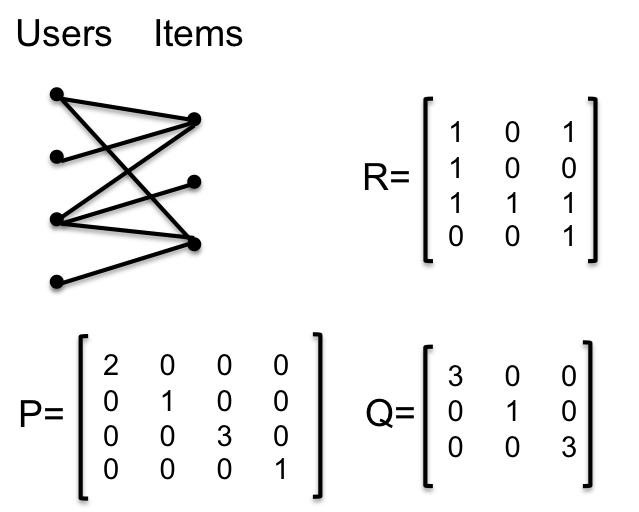
\includegraphics{user_item.png}
\caption{User-Item bipartite graph.}
\label{figpath}
\end{center}
\end{figure}

\vspace{0.4in}
\textbf{Cosine Similarity:} Recall that the cosine similarity of two vectors $u$
and $v$ is defined as:
\[ \textit{cos-sim(u,v)} = \frac {u \cdot v}{\|u\|\|v\|} \]

\subquestion{(b) [6 points]}

Let's define the \textit{item similarity matrix}, $S_{I}$, $n \times n$, such
that the element in row $i$ and column $j$ is the cosine similarity of \textit{item}
$i$ and \textit{item} $j$ which correspond to column $i$ and column $j$ of the matrix $R$. 
Show that $S_I = Q^{-1/2}R^TRQ^{-1/2}$, where $Q^{-1/2}$ is defined by $Q^{-1/2}_{rc} = 1/\sqrt{Q_{rc}}$ for all nonzero entries of the matrix, and $0$ at all other positions.

Repeat the same question for \textit{user similarity matrix}, $S_{U}$ where the
element in row $i$ and column $j$ is the cosine similarity of {\em user $i$} and
{\em user $j$}  which correspond to row $i$ and row $j$ of the matrix $R$. That is,
your expression for $S_U$ should also be in terms of some combination of $R$,
$P$, and $Q$. Your answer should be an operation on the matrices, in particular
you should not define each coefficient of $S_U$ individually.

Your answer should show how you derived the expressions.

\textit{(Note: To make the element-wise square root of a matrix, you may write it as matrix to the power of $\frac{1}{2}$.)}

\subquestion{(c) [5 points]}

The recommendation method using user-user collaborative filtering for user $u$, can be
described as follows: for all items $s$, compute $r_{u,s}=\Sigma_{x \in
\textit{users}}\cossim(x,u)*R_{xs}$ and recommend the $k$ items for which
$r_{u,s}$ is the largest.

Similarly, the recommendation method using item-item collaborative filtering for user $u$ can
be described as follows: for all items $s$, compute $r_{u,s}=\Sigma_{x \in
\textit{items}}R_{ux}*\cossim(x,s)$ and recommend the $k$ items for which $r_{u,s}$ is the largest.

Let's define the recommendation matrix, $\Gamma$, $m \times n$, such that
$\Gamma(i,j) = r_{i,j}$. Find $\Gamma$ for both item-item and user-user
collaborative filtering approaches, in terms of $R$, $P$ and $Q$. Your final answer should describe operations on matrix level, not specific terms of matrices. 

{\em Hint: For the item-item case, $\Gamma = RQ^{-1/2} R^TRQ^{-1/2}$.}

Your answer should show how you derived the expressions (even for the item-item case,
where we give you the final expression).

\subquestion{(d) [10 points]} In this question you will apply these methods to a real dataset. The data contains information about TV shows. More precisely, for 9985 users and 563 popular TV shows, we know if a given user watched a given show over a 3 month
period.

Use the dataset from \texttt{q4/data} within the bundle for this problem.

The folder contains:
\begin{itemize}
\item{\verb+user-shows.txt+} This is the ratings matrix $R$, where each row corresponds to a
user and each column corresponds to a TV show. $R_{ij} = 1$ if user $i$ watched the show
$j$ over a period of three months. The columns are separated by a space.
\item{\verb+shows.txt+} This is a file containing the titles of the TV shows, in the
same order as the columns of $R$.
\end{itemize}

We will compare the user-user and item-item collaborative filtering
recommendations for the 500\textsuperscript{th} user of the dataset. Let's call him Alex. (i.e. with Python's 0-based indexing, Alex=users[499].)

In order to do so, we have erased the first 100 entries of Alex's row in the
matrix, and replaced them by 0s. This means that we don't know which of the
first 100 shows Alex has watched. Based on Alex's behaviour on the other shows, we will give Alex recommendations on the first 100 shows. We will then see if our recommendations match what Alex had in fact watched.

\begin{itemize}
\item Compute the matrices $P$ and $Q$.
\item Using the formulas found in part (c), compute $\Gamma$ for the user-user
collaborative filtering. Let $S$ denote the set of the first 100 shows (the
first 100 columns of the matrix). From all the TV shows in $S$, which are the
five that have the highest similarity scores for Alex? In case of ties of similarity scores between two shows, choose the one with smaller index. Do not write the
index of the TV shows, write their names using the file \verb+shows.txt+.
\item Compute the matrix $\Gamma$ for the movie-movie collaborative filtering.
From all the TV shows in $S$, which are the five that have the highest similarity scores for
Alex? In case of ties between two shows, choose the one with smaller index.
Again, hand in the names of the shows and their similarity score.
\end{itemize}

For sanity check, your highest similarity score for user-user collaborative filtering should be above 900, and your highest similarity score for movie-movie filtering should be above 31. 

{\bf What to submit:} 
\begin{enumerate}[(i)]
\item Interpretation of $T_{ii}$ and $T_{ij}$ [4(a)]
\item Expression of $S_I$ and $S_U$ in terms of $R$, $P$ and $Q$ and accompanying explanation [4(b)]
\item Expression of $\Gamma$ in terms of $R$, $P$ and $Q$ and accompanying explanation [4(c)]
\item The answer to this question should include the followings: [4(d)]
\begin{itemize}
\item The \textbf{names} of five TV shows that have the highest similarity scores for Alex for the user-user collaborative filtering (no need to report the similarity scores)
\item The \textbf{names} of five TV shows that have the highest similarity scores for Alex for the item-item collaborative filtering (no need to report the similarity scores)
\item Upload the source code via Gradescope
\end{itemize}
\end{enumerate}

\end{document}
